\begin{frame} [fragile]
\small
	\frametitle{Method}
    		\begin{figure}
		 \centering
			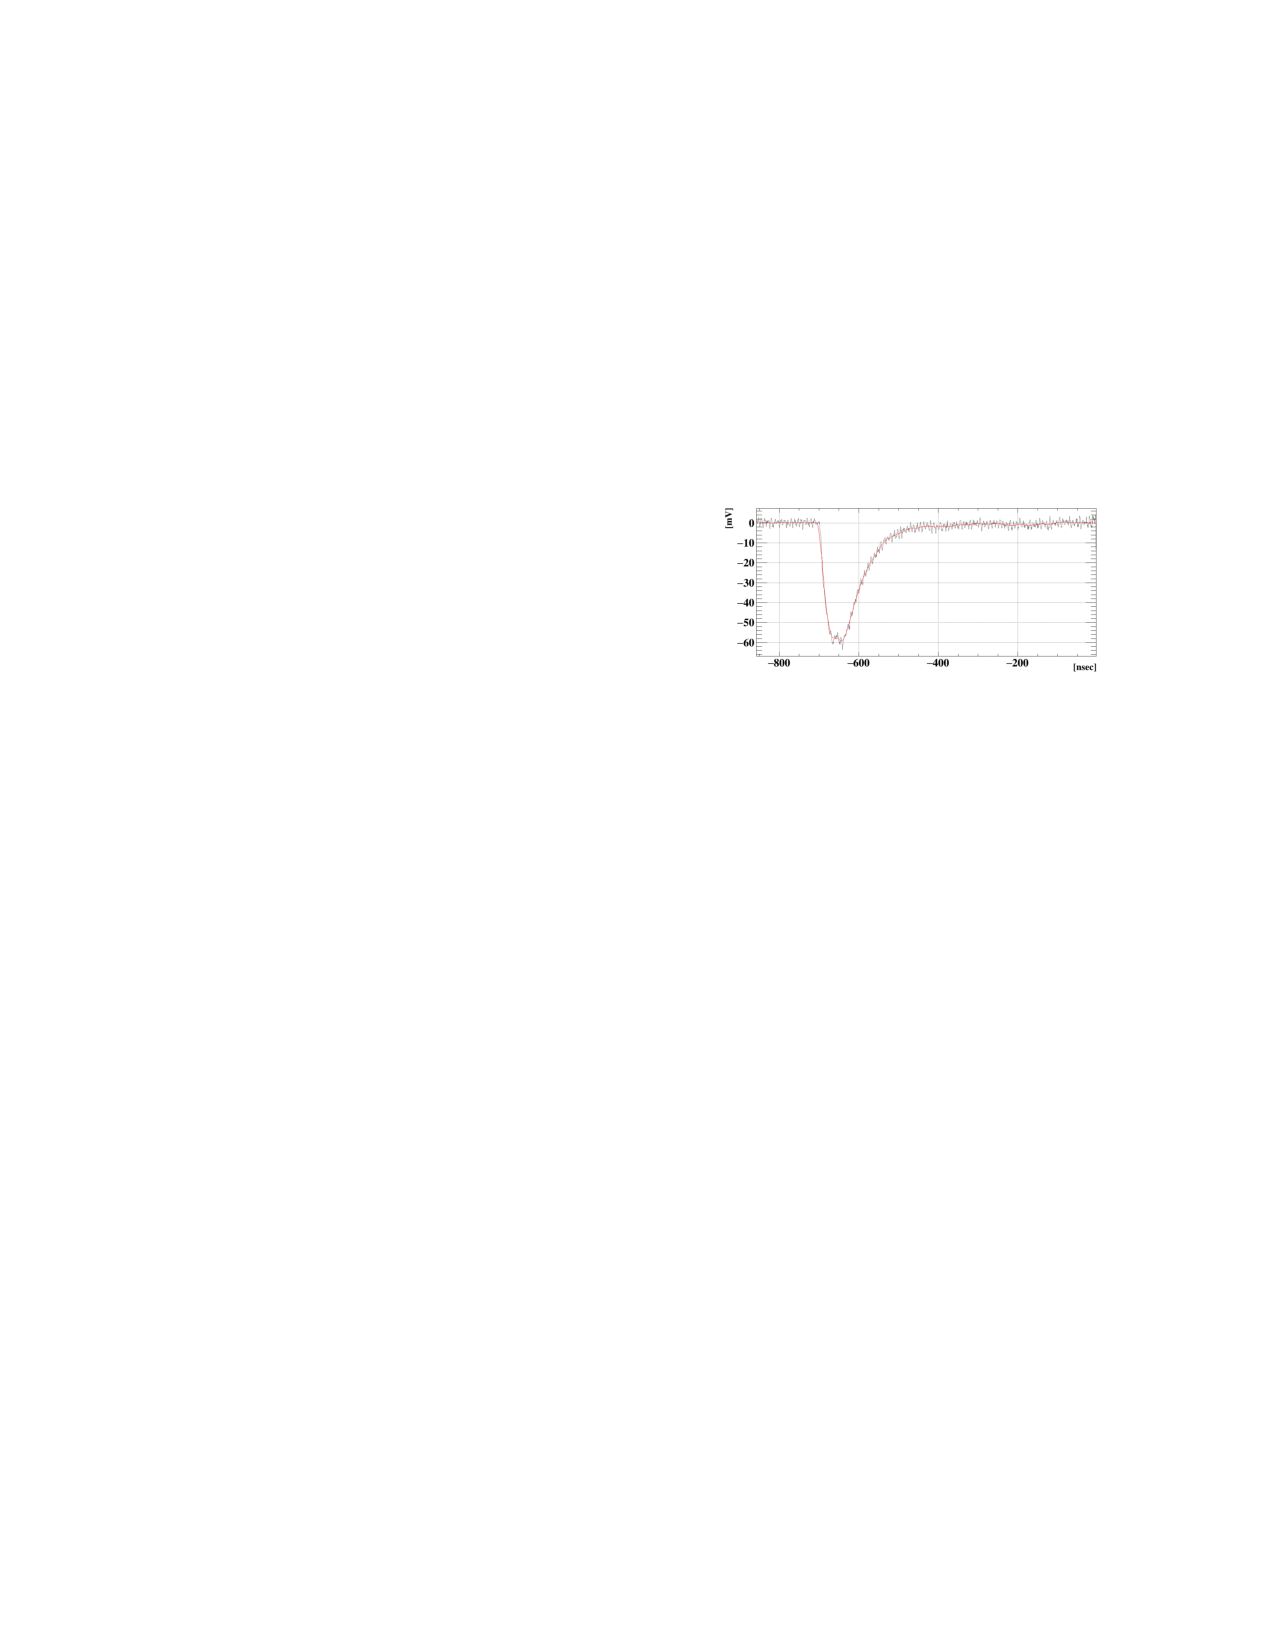
\includegraphics[scale=1.4]{figures/instruments/Waveform.pdf}
			\caption{Example Waveform recorded by DRS4}
		\end{figure}
	\begin{itemize}
		\item Select the \textcolor{blue}{channel} of interest (ch 0 $\longrightarrow$ 11)
		\item Measure the amplitude of the signal ($\pm$ 5 mV)
		\item Correlate with the \textcolor{red}{trigger value}  ($\pm$ 3 mV)
	\end{itemize}  
\end{frame}
